
\chapter{Метод исследования}

В работе движение жидкости моделируется численными решениями полных трехмерных уравнений Навье-Стокса. Все динамически существенные масштабы разрешаются явно, что освобождает от необходимости подбора замыкающих соотношений и эмпирических констант. Прямое численное моделирование зарекомендовало себя эффективным методом изучения пристенных турбулентных течений. Подробный численный анализ ряда пристенных течений показал, что численные решения уравнений Навье-Стокс с высокой точностью воспроизводят наблюдаемые в экспериментах особенности движения. Существенным достоинством численных методов при изучении механизмов турбулентности является то, что расчет дает полную информацию о течении. Изучаемые в работе переходные режимы течения наблюдаются при небольших значениях числа Рейнольдса (около 2000) и сегодня доступны для прямого численного моделирования даже на персональном компьютере. 

Значительный вклад в развитие численных методов решения задач гидродинамики внесли отечественные математики и механики. В работах Ольги Александровны Ладыженской обсуждаются вопросы разрешимости стационарных и нестационарных краевых задач для уравнений Навье-Стокса \cite{Lad1970}. В работах Виктора Иосифовича Юдовича дано обоснование методов линеаризации для решения задач гидродинамической устойчивости \cite{Jud1984}. Метод Галеркина для решения задач линейной устойчивости и расчета нелинейных режимов течения получил свое развитие в работах Георгия Ивановича Петрова и его учеников \cite{Petrov1940}. Исследованию задач устойчивости различных течений жидкости посвящены работы Виктора Яковлевича Шкадова \cite{Sch1973, Ach2009}, Григория Зиновьевича Гершуни и Ефима Михайловича Жуховицкого \cite{Ger1972}, Михаила Александровича Гольдштика и Владимира Николаевича Штерна \cite{Gold1977}. Некоторые принципы построения вычислительных алгоритмов предложены Константином Ивановичем Бабенко \cite{Bab2002}. Работы Семена Яковлевича Герценштейна посвящены исследованию конвективных течений \cite{Gerc1973, Gerc1975}. Моделирование процессов тепло и массообмена посвящены работы Вилена Михайловича Пасконова, Вадима Ивановича Полежаева, Льва Алексеевича Чудова \cite{Pask1984, Pol1987}. Олегом Михайловичем Белоцерковским предложена серия методов моделирования движения газа и жидкости и, в частности, турбулентных движений жидкости \cite{Bel1994}. Под руководством Бориса Леонидовича Рождественского в ИПМ им. Келдыша \cite{Rog1973, Rog1984, Pri1987, Rog1987} %\cite{Rog1973, Rog1984, -Rog1985, -Pon1988, Pri1987, -Pri1991, Rog1987, -Pri1992}
и Николаем Васильевичем Никитиным в НИИ механики МГУ \cite{Nikitin1994a, Nikitin1994b, Nikitin1996, Nikitin2006} разработаны методы для прямого численного моделирования движения жидкости в круглых трубах, плоских каналах и некоторых других геометриях течения, а также выполнены соответствующие расчеты. На западе наиболее интенсивные расчеты течения в плоском канале выполнены в группе под руководством Парвиза Моина в Стэнфордском университет \cite{Moin1978, Moin1982, Kim1987}. %Katasonov2014

Наиболее эффективные вычислительные алгоритмы разработаны для решения уравнений Навье-Стокса для несжимаемой жидкости в областях простой геометрической формы, в частности, в геометрии плоского канала и геометрии круглой трубы. В типичной постановке по продольной и поперечной координатам на решение накладывается условие периодичности. В круглой трубе период в поперечном направлении составляет $2\pi$, в плоском канале этот период может быть произвольным и является дополнительным параметром задачи. Такая постановка хорошо зарекомендовала себя при исследовании развитых турбулентных течений. Условия периодичности снимают необходимость установки входных и выходных условий (в плоском канале, также, условий в поперечном направлении) и исключает влияние конкретных входных и выходных условий на режим течения. В тоже время, увеличивая период, можно минимизировать влияние условия периодичности на характеристики потока. Характеристики развитых турбулентных течений, полученные в такой постановке, с большой точностью совпадают с экспериментальными данными \cite{Kim1987, Eggels1994, Nikitin1996}. Расчеты пространственно неоднородных турбулентных течений (турбулентных порывов) также проводятся в приведенной постановке и показывают согласие с экспериментальными данными \cite{Priymak2004, Avila2010, Song2017}. Для адекватного воспроизведения локализованных турбулентных структур необходимо выбирать длину периода достаточно большой для того, чтобы пространственная неоднородность течения могла проявить себя. Подход, при котором в продольном направлении устанавливается условие периодичности, называется временным. Альтернативный ему пространственный подход, при котором вместо условия периодичности в продольном направлении ставятся условия во входном и выходном сечениях, примененный для моделирования движения жидкости в круглой трубе в \cite{Nikitin1995}, требует значительно больших вычислительных ресурсов, но позволяет воспроизводить эволюцию возмущений, попадающих в поток во входном сечении, при их продвижении вниз по потоку. Согласно \cite{Nikitin1995}, при пространственном походе к моделированию течения в трубах в области, где режим течения устанавливается, характеристики течения согласуются с характеристиками, полученными при временном подходе. 

Общепринятым подходом при построении дискретной системы уравнений является представление решения в виде суммы рядов Фурье. При этом по продольной и поперечной координатам решение представляется суммой тригонометрических функций, а в нормальном к стенке направлении могут быть использованы полиномы Чебышева либо другие ряды \cite{Orszag1971b, Meseguer2007}. Дискретизация уравнений выполняется методом Галеркина, обоснованным в работе Г.И. Петрова \cite{Petrov1940}. При этом основная сложность алгоритма оказывается связана с вычислением нелинейных слагаемых, что требует свертки рядов. Наиболее эффективные алгоритмы, позволяющие вычислить свертку рядов, основаны на применении быстрого преобразования Фурье \cite{Cooley1965}. Альтернативным подходом является конечно-разностная дискретизация уравнений \cite{Nikitin2006}. Конечно-разностные методы уступают спектральным при моделировании предтурбулентных режимов течения, для которых свойственны достаточно гладкие поля скорости и отсутствие мелкомасштабной составляющей движения \cite{Orszag1971a}, однако в развитых турбулентных течениях число гармоник Фурье и число точек в сетке, необходимые для того, чтобы достаточно точно приблизиться поле скорости, оказываются сравнимы, и конечно-разностные методы не уступают спектральным в эффективности \cite{Rai1991}. К преимуществам конечно-разностных методов можно отнести то, что они достаточно просты в реализации, сравнительно легко адаптируются к изменению геометрии расчетной области и граничных условий. Также распространены методы, в которых в продольном и поперечном направлении решения представляются в виде суммы тригонометрических рядов, а в нормальном к стенке направлении дискретизация выполняется конечно-разностным методом \cite{Nikitin1994a}.

В настоящей работе движение жидкости в трубе описывается решениями уравнений Навье-Стокса для несжимаемой жидкости. Уравнения решаются в цилиндрической расчетной области с условием периодичности вдоль потока. Дискретизация уравнений выполняется конечно-разностным методом, разрабатываемым Н.В. Никитиным \cite{Nikitin2006}. Этот метод применялся для решения большого числа задач и хорошо себя зарекомендовал \cite{Yakhot2006a, Yakhot2006b, Holzner2008, Demekhin2013}. 

\section{Постановка задачи} \label{math_section}

Рассматривается движение вязкой несжимаемой жидкости в прямой трубе круглого сечения. Движение жидкости описывается уравнениями Навье-Стокса и неразрывности:
\begin{equation} \label{NS_eq}
\pd{\v}{t} = - (\v \cdot \nabla) \v - \frac{1}{\rho}\grad p + \nu \nabla^2 \v,
\end{equation}
\begin{equation} \label{div_eq}
\nabla \cdot \v = 0.
\end{equation}
Здесь $\v$ --- поле скорости, $p$ --- давление, $\rho$ и $\nu$ --- постоянные плотность жидкости и кинематический коэффициент вязкости, $t$ --- время. 

Задача решается в цилиндрической системе координат $(x,r,\theta)$. На стенках трубы, имеющей радиус $R$, ставится условие прилипания:
\begin{equation} \label{bc1_eq}
\v \big|_{r=R} = 0.
\end{equation}
В продольном направлении на поле скорости накладывается условие периодичности с периодом $L_x$:
\begin{equation} \label{bc2_eq}
\v \big|_{x+L_x} = \v \big|_{x}.
\end{equation}
Давление в этом случае имеет вид:
$$
p = - D_p(t)x + q, \ \ \ \  q\big|_{x+L_x} = q\big|_{x},
$$
где $D_p$ --- внешний градиент давления, вызывающий движение жидкости. 

Значение $D_p$ определяется из условия постоянства расходной скорости $U_m$, которая, в свою очередь, определяется начальным условием:
$$
\v\big|_{t=0} = \v_0.
$$

 
Задача решается в безразмерных переменных. В качестве основных единиц измерения выступают радиус трубы $R$, максимальная скорость течения Пуазейля $U = 2U_m$ и плотность жидкость $\rho$. Безразмерным параметром системы является число Рейнольдса:
$$
\Re = \frac{R U}{\nu}. 
$$

Задача поставлена традиционным образом для прямого расчета развитых турбулентных течений в трубах и каналах. В такой постановке удается воспроизводить характеристики течения, устанавливающегося на большом удалении от входа в трубу, решая уравнения движения в ограниченной расчетной области. Условие периодичности вдоль трубы освобождает от необходимости устанавливать условия на входе и выходе из трубы. В тоже время, увеличивая длину периода $L_x$, можно минимизировать влияние этого условия на поток. Для того, чтобы иметь возможность воспроизвести в расчете локализованные турбулентные структуры, необходимо выбирать протяженность расчетной области $L_x$ достаточно большой, не менее $40$ диаметров трубы. 

\section{Численный метод} \label{num_method}

Задача решается конечно-разностным методом, наиболее полно описанным в \cite{Nikitin2006}. Численный метод формулируется относительно уравнения движения \eqref{NS_eq}, преобразованного к	 виду:
\begin{equation}\label{NSom_eq}
\pd{\v}{t} =  \v \times \om  - \grad \Pi - \nu \rot \om,
\end{equation}
где $\om = \rot \v$ --- вектор завихренности, $\Pi = p/\rho + \v^2/2$ --- полное кинематическое давление. Эквивалентность уравнений \eqref{NS_eq} и \eqref{NSom_eq} следует из несжимаемости жидкости и векторных тождеств:
\begin{equation*}
-(\v \cdot \nabla) \v = \v \times \rot \v - \grad \frac{\v^2}{2},
\end{equation*}
\begin{equation*}
\nabla^2 \v = \nabla (\nabla \cdot \v) - \rot \rot \v.
\end{equation*}

Дискретизация по направлениям $x$, $r$, $\theta$ проводится независимым образом. По координатам $x$ и $\theta$ сетка однородна. Расстояние между соседними узлами в направлениях $x$ и $\theta$ равно $h_x = L_x / N_x$ и $h_\theta  = 2 \pi / N_\theta$, где $N_x$ и $N_\theta$ --- количество ячеек в соответствующих направлениях. В нормальном к стенке направлении вводится растяжение сетки, что позволяет сгустить сетку вблизи стенки, где наблюдаются наибольшие градиенты скорости. Во всех расчетах параметр растяжения выбран таким образом, что высота ячеек вблизи стенки в 4 раза меньше, чем в центре трубы. Число ячеек в радиальном направлении равно $N_r$. При дискретизации различные скалярные величины отнесены к различным точкам сетки. Давление $p$ относится к центру ячеек. Компоненты вектора скорости $v_i$ относятся к центрам граней, нормальных к направлению $i$. Компоненты вектора завихренности $\omega_i$ относятся к центрам ребер, параллельных направлению $i$. При таком подходе говорят, что неизвестные определены на смещенных или разнесенных сетках. 

Дискретная система уравнений обладает рядом важных консервативных свойств. В частности, дивергенция поля завихренности в расчете тождественно равна нулю. Дискретный аналог ротора градиента давления тождественно равен нулю, что гарантирует, что давление не оказывает влияния на эволюцию поля завихренности напрямую. Дискретный аналог дивергенции вязкого слагаемого в уравнении Навье-Стокса тождественно равна нулю, что гарантирует, что это слагаемое не производит массы. 

При моделировании турбулентных течений важно аккуратно воспроизводить изменение кинетической энергии системы. Описывающее его уравнение возникает в результате скалярного умножения на $\v$ уравнений движения с последующим суммированием по всей расчетной области. Важным свойством системы является то, что градиент периодической составляющей давления $q$ и нелинейные слагаемые не производят кинетической энергии, а лишь перераспределяют ее внутри объема жидкости. Это свойство выражается тождествами:
$$
\int_V \v \cdot \grad q\ d\tau= \int_V \grad (\v q)\ d\tau = \int_{\Sigma} q v_n\ d\sigma = 0, 
$$
$$
\int_V \v \cdot (\v \cdot \nabla) \v\ d\tau = \int_V (\v \cdot \nabla)\frac{\v^2}{2}\ d\tau = \int_V \grad (\v \frac{\v^2}{2}) d\tau = \int_{\Sigma} \frac{\v^2}{2} v_n d\sigma = 0,
$$
где $V$ --- расчетная область, $\Sigma$ --- её граница, $d\tau$ и $d\sigma$ --- малые элементы объема и границы, $v_n$ --- нормальная составляющая скорости на границе. Справедливость тождеств следует из условия несжимаемости и условий прилипания на твердой стенке \eqref{bc1_eq} и периодичности вдоль потока \eqref{bc2_eq}. Строго выполняется дискретный аналог уравнения изменения кинетической энергии $E$, записанного в виде:
$$
\frac{d E}{d t} = U_mVD_p - \nu \int_{V} \om^2 d\tau,
$$
$$
E = \frac{1}{2}\int_{V} \v^2 d\tau.
$$
Здесь $V$ обозначает также объем области, по которой выполняется интегрирование. Изменение кинетической энергии происходит за счет внешнего градиента давления $D_p$ и вязкой диссипации. 

Для определения давления решается уравнение Пуассона, возникающее в результате применения оператора дивергенции к уравнению движения \eqref{NSom_eq} с учетом того, что жидкость несжимаемая. Уравнение для определения давления имеет вид:
\begin{equation}\label{Pres_eq}
\nabla^2 \Pi = \div \tilde \v,
\end{equation}
\begin{equation}\label{tildev_eq}
\tilde \v =  \v \times \om - \nu \rot \om.
\end{equation}
Правая часть уравнения \eqref{Pres_eq} определяется полем скорости $\v$, которое в данном случае считается известным. Условие на твердой стенке возникает в результате проектирования уравнения \eqref{NSom_eq} на направление нормали $n$ и имеет вид:
\begin{equation}\label{Pbc_eq}
\pd{\Pi}{n} = \tilde v_n,
\end{equation}
где $\tilde v_n$ --- нормальная к стенке составляющая вектора $\tilde\v$, определенного в \eqref{tildev_eq}. В процессе решения задачи сперва ищется периодическая вдоль потока составляющая движения, также как и $\Pi$, удовлетворяющая \eqref{Pres_eq} и \eqref{Pbc_eq}. Затем внешний градиент давления $D_p$ определяется из условия постоянства средней скорости. 


Простая геометрия расчетной области позволяет применять прямые методы решения возникающей в результате дискретизации уравнения \eqref{Pres_eq} линейной системы. Метод решения задачи для давления основан на применении быстрого преобразования Фурье в направлениях $x$ и $\theta$, в которых решение меняется периодическим образом и сетка имеет постоянный шаг. В радиальном направлении система решается методом прогонки. Общая сложность решения задачи для давления составляет $O(N_x N_r N_\theta \log N_x N_\theta)$. Решение задачи для давления составляет основную вычислительную сложность используемого метода. 

Дискретная система уравнений при достаточно высоком пространственном разрешении оказывается жесткой и требует неявных методов интегрирования по времени. Наиболее эффективными методами интегрирования по времени при моделировании турбулентных потоков являются полунеявные методы, в которых только часть оператора Навье-Стокса разрешается неявно. В работе применяется полунеявный метод Рунге-Кутты третьего порядка точности, описанный в \cite{Nikitin2006third}, в котором неявно разрешается вязкое слагаемое (линейное). Именно с этим слагаемым связана основная жесткость системы. На каждом шаге по времени метод дает два приближения к решению, с третьим и с четвертым порядками точности, что позволяет, контролируя разность между двумя приближениями, автоматически выбирать шаг интегрирования по времени. 


\section{Реализация численного метода}

Пакет программ, реализующих описанный в предыдущем разделе численный метод, написан на языке программирования fortran77 Н.В.\,Никитиным. Численный метод используется как в лаборатории общей аэродинамики института механики МГУ, так и в других местах в разных частях света уже более 20 лет и хорошо себя зарекомендовал. Программный код отлажен в процессе решения большого числа задач. В частности, с его помощью получены результаты, приведенные в работе \cite{Nikitin2006}, демонстрирующие согласие характеристик турбулентных потоков, полученных численно и в экспериментах. Адекватность численного метода и качество его программной реализации подтверждают также результаты расчетов течения жидкости в трубе при переходных $\Re$, приведенные в следующем разделе. В соответствии с результатами эксперимента, в расчетах турбулентность принимает форму локализованных структур, характеристики которых совпадают с характеристиками турбулентного порыва.

Помимо последовательного варианта программы реализован параллельный, позволяющий выполнять расчеты на кластерных вычислительных системах с распределенной памятью. Для коммуникации между процессами, запущенными на различных узлах вычислительной системы, использован интерфейс передачи сообщений MPI (<<Message Passing Interface>>). Значительная часть расчетов выполнена на суперкомпьютерах <<Чебышев>> и <<Ломоносов>> суперкомпьютерного комплекса МГУ. 

Значительная часть кода, необходимого при анализе полученных результатов и управлении численными экспериментами, в том числе реализующая метод поиска решения на сепаратрисе (см. раздел \ref{edge_seq}) и метод поиска условно периодических траекторий (см. раздел. \ref{Newton_seq}), была написана на высокоуровневом языке python автором диссертации. Применение указанных методов сводится к последовательному обращению к программе расчета движения жидкости с правильно сформированными начальными данными. 


\section{Методические расчеты} \label{puff_calc}

В разделе приведены результаты расчетов движения жидкости в круглой трубе в диапазоне $1670 \leqslant \Re \leqslant 2800$, полученные при $L_x=200R$ с пространственным разрешением $2048 \times 64 \times 128$ ячеек в продольном, радиальном и угловом направлении соответственно. Расчеты на более грубой сетке $1024 \times 32 \times 64$ во всех рассмотренных случаях дают результаты совпадающие качественно и близкие количественно.

\begin{figure}[h]
\center{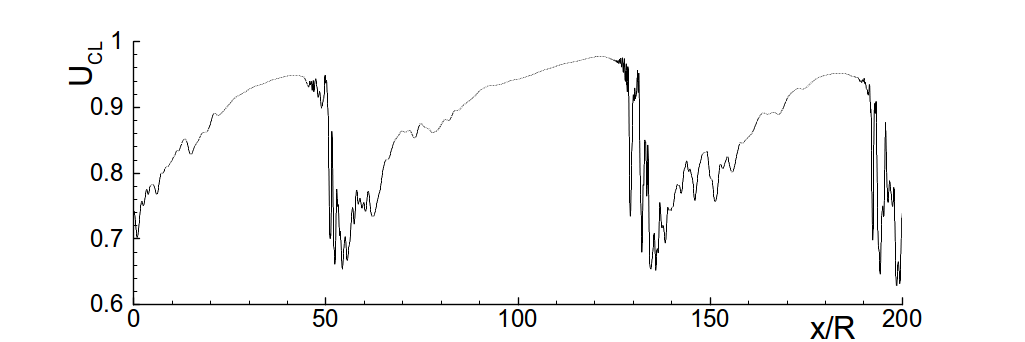
\includegraphics[width=0.9\linewidth]{exper2.png}}
\center{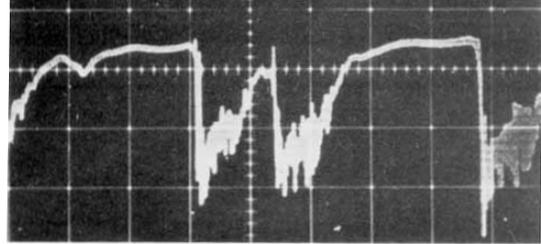
\includegraphics[width=0.68\linewidth]{exper3.png}}
\caption{Сравнение результатов численного расчета и эксперимента. Изображен график скорости на оси трубы. Верхний график построен по результатам численного моделирования, выполнено Н.В. Никитиным применяемым в работе методом. Нижний график получен в эксперименте \cite{Wygnanski1973}.}
\label{exper_img}
\end{figure}

Стартуя с начальных данных в виде некоторого трехмерного возмущения течения Пуазейля, уравнения Навье--Стокса интегрируются до выхода решения на тот или иной режим. Установление решения, отвечающего турбулентному течению, происходит в том случае, когда амплитуда начального возмущения достаточно велика, в противном случае возмущения затухают со временем, и решение в конечном итоге возвращается к ламинарному течению Пуазейля. Турбулентный режим за пределами диапазона переходных чисел Рейнольдса $\Re \geqslant 3000$ имеет вид статистически стационарного процесса и не зависит от конкретного вида начальных условий, при которых он был получен. Течение при этом однородно в продольном направлении, его статистические характеристики согласуются с имеющимися экспериментальными данными. При $\Re \leqslant 2600$ в распределении скорости вдоль трубы появляется неоднородность, которая при $\Re \lesssim 2200$ приобретает форму двигающейся вдоль трубы цепочки из нескольких пространственно-локализованных структур, разделенных участками ламинарного течения. Конкретное число получающихся в решении турбулентных структур зависит от начальных условий. Кроме того, как было отмечено выше, это число может меняться в процессе эволюции в результате исчезновения или деления отдельных структур. Получаемые в расчетах пространственно-локализованные турбулентные структуры хорошо согласуются с наблюдаемыми в экспериментах турбулентными порывами, что позволяет нам пользоваться этим их наименованием (смотри Рисунок \ref{exper_img}). Отметим, что турбулентные порывы формируются и на некотором отрезке времени существуют в расчетах и при $\Re < 2000$. Однако, в этом случае не только число порывов в пределах расчетной области, но и время их существования является случайной величиной и зависит от конкретных начальных условий. Представленная на фиг.~\ref{puffs_img} визуализация рассчитанных течений в диапазоне $1680 \leqslant \Re \leqslant 2800$ демонстрирует изменение локализованных структур при уменьшении числа Рейнольдса.

\begin{figure}[h]
\center{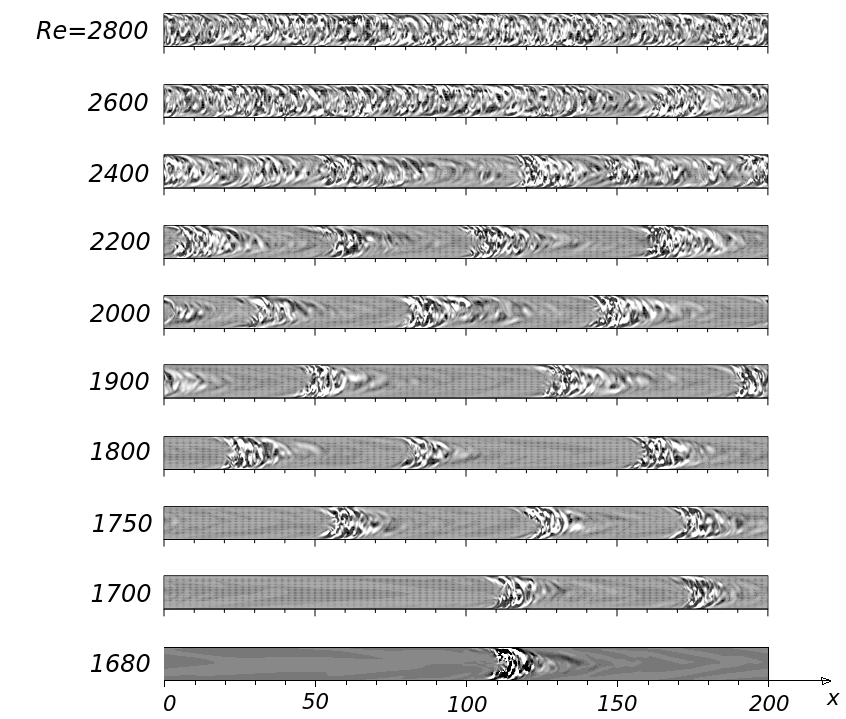
\includegraphics[width=1\linewidth]{puffs.png}}
\caption{Перемежаемый характер турбулентности в трубе в диапазоне переходных чисел Рейнольдса.}
\label{puffs_img}
\end{figure}


\begin{comment}
Задача решается конечно-разностным методом, наиболее полно описанным в \cite{Nikitin2006}. Все величины представляются в безразмерном виде. В качестве единиц измерения выступают радиус трубы $R$, максимальная скорость течения Пуазейля (удвоенная средняя скорость течения) $U$, плотность жидкость $\rho$ и кинематический коэффициент вязкости $\nu$. Численный метод формулируется относительно уравнения движения \eqref{NS_eq}, преобразованного к виду:
\begin{equation}\label{NSom_eq}
\pd{\v}{t} =  \v \times \om  - \grad \Pi - \frac{1}{\Re} \rot \om,
\end{equation}
где $\om = \rot \v$ --- вектор завихренности, $\Pi = p/\rho + \v^2/2$. Эквивалентность уравнений \eqref{NS_eq} и \eqref{NSom_eq} следует из несжимаемости жидкости и векторных тождеств:
\begin{equation*}
-(\v \cdot \nabla) \v = \v \times \rot \v - \grad \frac{\v^2}{2},
\end{equation*}
\begin{equation*}
\nabla^2 \v = \nabla (\nabla \cdot \v) - \rot \rot \v.
\end{equation*}

В скалярных переменных уравнения \eqref{NSom_eq} и \eqref{div_eq} имеют вид:
\begin{equation}\label{NS_scalar_eq}
\pd{v_x}{t} = \left( v_r \omega_\theta - v_\theta \omega_r \right) - \pd{\Pi}{x} - \frac{1}{\Re} \left(\frac{\partial r\omega_\theta}{r\partial r} - \frac{\partial \omega_r}{r \partial \theta}\right),
\end{equation}
\begin{equation}
\pd{v_r}{t} = \left( v_\theta \omega_x - v_x \omega_\theta \right) - \pd{\Pi}{r} - \frac{1}{\Re} \left(\frac{\partial \omega_x}{r \partial \theta} - \frac{\partial \omega_\theta}{\partial x}\right),
\end{equation}
\begin{equation}
\pd{v_\theta}{t} = \left( v_x \omega_r - v_r \omega_x \right) - \frac{1}{r}\pd{\Pi}{\theta} - \frac{1}{\Re} \left(\pd{\omega_r}{x} - \pd{\omega_x}{r}\right),
\end{equation}
\begin{equation}
\frac{1}{r} \left( \pd{rv_x}{x} + \pd{rv_r}{r} + \pd{v_\theta}{\theta}\right) = 0.
\end{equation}
Здесь $(v_x, v_r, v_\theta)$ --- компоненты вектора скорости, $(\omega_x, \omega_r, \omega_\theta)$ --- компоненты вектора завихренности, вычисляемые по формулам:
\begin{equation}
\omega_x = \frac{1}{r}\left(\pd{r v_\theta}{r} - \pd{v_r}{\theta}\right), 
\end{equation}
\begin{equation}
\omega_r = \frac{1}{r}\left(\pd{v_x}{\theta} - \pd{rv_\theta}{x}\right), 
\end{equation}
\begin{equation}\label{om_scalar_eq}
\omega_\theta = \pd{v_r}{x} - \pd{v_x}{r}.
\end{equation}

Расчетная область $D$, в которой решаются уравнения \eqref{NS_scalar_eq}--\eqref{om_scalar_eq}, имеет форму цилиндра высоты $L_x$:
\begin{equation}
D = \{ 0 \le x \le L_x, 0 \le r \le 1, 0 \le \theta \le 2\pi \}. 
\end{equation}
Дискретизация уравнений по координатам $x$, $r$, $\theta$ производится независимым образом. По координатам $x$ и $\theta$ сетка однородна, расстояние между узлами сетки равно $h_x = L_x / M$ и $h_\theta = 2\pi / K$, где $M$ и $K$ --- число ячеек сетки в направлениях $x$ и $\theta$. В радиальном направлении сетка неоднородна. 



Все пространственные производные 
Расчетная сетка имеет вид 
В пространстве $(x,r,\theta)$ в расчетной области вводится прямоугольная расчетная сетка, однородная в направлениях $x$ и $\theta$. В радиальном направлении вводится растяжение сетки, что позволяет уменьшить её шаг вблизи стенки. Во всех расчетах, представленных в работе, параметр растяжения выбран таким образом, что размер ячейки в радиальном направлении около стенки в 4 раза меньше, чем в центре трубы. 


\begin{equation}\label{NS_scalar_eq}
\pd{v_x}{t} = \frac{1}{r}\left( \overline{\overline{v_r}^x r \omega_\theta}^r - \overline{\overline{r v_\theta}^x \omega_r}^\theta \right) - \pd{\Pi}{x} - \frac{1}{\Re} \left(\frac{\delta r\omega_\theta}{r \delta r} - \frac{\delta \omega_r}{r \delta \theta}\right),
\end{equation}
\begin{equation}
\pd{v_r}{t} = \frac{1}{r}\left( \overline{\overline{r v_\theta}^r \omega_x}^\theta - \overline{\overline{v_x}^r r \omega_\theta}^x \right) - \pd{\Pi}{r} - \frac{1}{\Re} \left(\frac{\delta \omega_x}{r \delta \theta} - \frac{\delta r \omega_\theta}{r \delta x}\right),
\end{equation}
\begin{equation}
\pd{v_\theta}{t} = \left( v_x \omega_r - v_r \omega_x \right) - \frac{1}{r}\pd{\Pi}{\theta} - \nu \left(\pd{\omega_r}{x} - \pd{\omega_x}{r}\right),
\end{equation}
\begin{equation}
\frac{1}{r} \left( \pd{rv_x}{x} + \pd{rv_r}{r} + \pd{v_\theta}{\theta}\right) = 0.
\end{equation}
Здесь $(v_x, v_r, v_\theta)$ --- компоненты вектора скорости, $(\omega_x, \omega_r, \omega_\theta)$ --- компоненты вектора завихренности, вычисляемые по формулам:
\begin{equation}
\omega_x = \frac{1}{r}\left(\pd{r v_\theta}{r} - \pd{v_r}{\theta}\right), 
\end{equation}
\begin{equation}
\omega_r = \frac{1}{r}\left(\pd{v_x}{\theta} - \pd{rv_\theta}{x}\right), 
\end{equation}
\begin{equation}\label{om_scalar_eq}
\omega_\theta = \pd{v_r}{x} - \pd{v_x}{r}.
\end{equation}
\end{comment}


